%!Tex root = Linguaggi.tex

\chapter{Introduzione}
Il problema principale dell'informatica consiste nel voler far eseguire a una macchina algoritmi che manipolano dati.

\[
    \text{macchina} \xrightarrow{\textcolor{red}{\textbf{esegue}}} \text{algoritmo} \xrightarrow{\textcolor{red}{\textbf{manipolazione}}} \text{dati}
\]

Il primo meccanismo che viene associato alla storia dei computer è la \textbf{macchina di Babbage}, che può essere visto come il primo "computer" perchè nasce per eseguire calcoli matematici complessi in modo automatico.

\smallskip
Sucessivamente, c'è un'evoluzione e il computer viene riconosciuto come macchina programmabile (dare delle istruzioni alla macchina per ottenere un determinato risultato).\\[0.2ex]
In questo contesto nasce \textbf{Enigma}, uno strumento per decodificare un codice mediante un algoritmo di forza bruta che tenta tutte le combinazioni.

La prima architettura che darà origine all'architettura dei computer moderni è l'\textcolor{colore}{\textbf{architettura di Von Neumann}}, un'architettura hardware che comprende solo il linguaggio binario (costituito da stringhe di bit 0 e 1) e che può essere utilizzato per codificare qualunque altro linguaggio, ma non è comprensibile dall'essere umano.\\[0.2ex]
Questo fa si che l'uomo per poter interagire e programmare macchine, necessita di un'evoluzione dei linguaggi, ha bisogno di costruire un linguaggio comprensibile in modo più immediato.

\section{Perchè studiare i PL?}
Le motivazioni sono diverse:
\begin{itemize}[label=$\triangleright$, itemsep=\smallskipamount]
    \item migliorare la capacità di esprimere idee in forma algoritmica
    \item scegliere appropriatamente un linguaggio
    \item migliorare la capacità di studiare o progettare nuovi linguaggi o costrutti
    \item comprendere meglio il significato dell'implementazione dei linguaggi di programmazione
\end{itemize}

\section{Cosa sono i PL?}
La nascita e l'evoluzione dei linguaggi di programmazione è, anche, dovuto all'architettura della macchina che bisogna programmare.

I computer moderni nascono dall'archiettura di Von Neumann.\\[0.2ex]
Questa è una tipologia di architettura hardware con programma memorizzato, dove \textbf{dati} e \textbf{istruzioni} condividono la stessa area di memoria.

\begin{figure}[H]
    \centering
    \includegraphics[width=0.6\textwidth]{images/architettura-von-neumann.png}
\end{figure}

\section{Cosa significa programmare?}
Il linguaggio di programmazione deve essere uno strumento che permette di descrivere algoritmi e rappresentare i dati.

\begin{figure}[H]
    \centering
    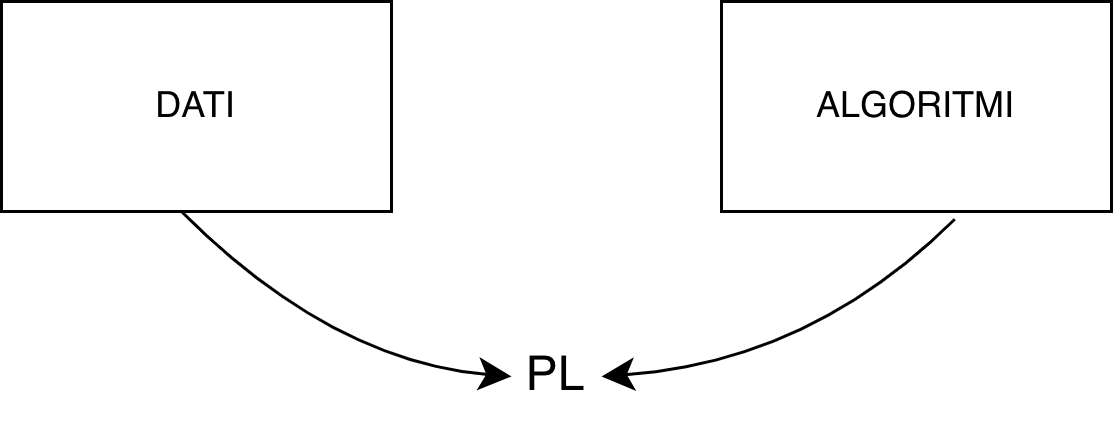
\includegraphics[width=0.5\textwidth]{images/linguaggio-programmazione.png}
\end{figure}

Il linguaggio binario è un linguaggio di programmazione in quanto permette di rappresentare algoritmi e dati, ma non è umanamente utilizzabile o interpretabile, in quanto un'istruzione potrebbe essere usata come dato o un dato interpretato come istruzione.\\[0.2ex]
Ciò significa, che un linguaggio di programmazione deve permettere di superare queste difficoltà, fornendo una chiara distinzione tra dato e istruzione.

\begin{mydef}{algoritmo}
    Un \textbf{algoritmo} è una sequenza infinta di passi di computazione, ovvero scompone un calcolo complesso in passi elementari.
\end{mydef}

Un algoritmo è un concetto astratto che trova forma concreta in un programma (sequenza finita di istruzioni).

\begin{mydef}{dati}
    I \textbf{dati} sono informazioni memorizzate concretamente in celle di memoria e astratte in elementi che il linguaggio può manipolare (variabili).
\end{mydef}

\begin{mydef}{programma}
    Un \textbf{programma} è la concretizzazione di un algoritmo che manipola dati.
\end{mydef}

\begin{mydef}{linguaggio di programmazione}
    Un \textbf{linguaggio di programmazione} è una notazione per scrivere un programma (serve a dare forma concreta agli algoritmi).
\end{mydef}

Il programma, quindi, costituisce la \textcolor{colore}{\textbf{sintassi}}.

\smallskip
Un programma è necessariamente un oggetto finito (sempre concreto), mentre il calcolo di una funzione richiede l'esecuzione di un insieme di passi primitivi, che, però, possono essere infiniti.\\[0.2ex]
Ciò significa che un programma è una rappresentazione finita di un insieme, potenzialmente infinito, di passi primitivi di computazione.

\vario{Nota}{
    I linguaggi di programmazione devono dare specifica finita di oggetti potenzialmente infiniti.
}

\section{Contesti di sviluppo}
Il contesto in cui il linguaggio deve operare determina le funzionalità che deve gestire efficacemente:
\begin{itemize}[label=$\triangleright$, itemsep=\smallskipamount]
    \item \textbf{applicazioni scentifiche} (es. $\verb|Fortran|$)
    \item \textbf{applicazioni economiche} (es. $\verb|COBOL|$)
    \item \textbf{applicazioni artificiali} (es. $\verb|LISP|$)
    \item \textbf{programmazione di sistemi} (es. $\verb|C|$)
    \item \textbf{web software} (es. $\verb|HTML|$ (markup), $\verb|PHP|$ (scripting), ecc.)
\end{itemize}

\section{Classificazione dei PL}
I linguaggi di programmazione si possono classificare in:
\begin{itemize}[label=$\diamond$, itemsep=\smallskipamount]
    \item \textcolor{colore}{\textbf{basso livello}}: linguaggi con caratteristiche specifiche dipendenti dall'architettura che si sta programmando (es. $\verb|linguaggio binario|$, $\verb|Assembly|$)
    \item \textcolor{colore}{\textbf{alto livello}}: linguaggi che permettono una programmazione strutturata in cui dati e istruzioni hanno rappresentazioni diverse
\end{itemize}

I linguaggi ad alto livello si possono classificare in base a:
\begin{itemize}[label=$\circ$, itemsep=\medskipamount]
    \item \textbf{paradigma di programmazione}
    \begin{itemize}[itemsep=\smallskipamount]
        \item linguaggi procedurali: codice diviso in sub-rutine che eseguono compiti semplici basati su salti condizionali (goto) [es. $\verb|COBOL|$]
        \item linguaggi strutturati (imperativi): procedurale senza goto (es. $\verb|C|$, $\verb|Pascal|$, $\verb|ADA|$, ec..)
        \item linguaggi orientati agli oggetti: classe elemento centrale della programmazione.
        
        Un linguaggio deve avere tre proprietà:
        \begin{itemize}[itemsep=\smallskipamount]
            \item incapsulamento
            \item eriditarietà
            \item polimorfismo
        \end{itemize}
        \item linguaggi dichiatirativi: basati su componenti della matematica
        \begin{itemize}[itemsep=\smallskipamount]
            \item logici: basati sulla logica proposizionale del primo ordine, in cui si effettuano calcoli tramite dimostrazione di fatti (es. $\verb|PROLOG|$)
            \item matematici: basati sul concetto di applicazione di funzione (es. $\verb|LSIP|$, $\verb|ML|$)
        \end{itemize}
    \end{itemize}
    \item \textbf{termini gerazionali}
    \begin{itemize}[itemsep=\smallskipamount]
        \item I° generazione: basso livello, linguaggi proprietari HW
        \begin{center}
            $\downarrow \textcolor{red}{\text{astrazione}}$
        \end{center}
        \item II° generazione: basso livello (\texttt{Assembly})
        \begin{center}
            $\downarrow \textcolor{red}{\text{avvicinamento al linguaggio naturale}}$
        \end{center}
        \item III° generazione: \texttt{C}
        \begin{center}
            $\downarrow \textcolor{red}{\text{cambio di prospettiva}}$
        \end{center}
        \item IV° generazione: uso della matematica (linguaggi dichiatirativi) [\texttt{SQL}]
        \begin{center}
            $\downarrow$
        \end{center}
        \item V° generazione: non semplice esecuzione di programmi scritti e fissati
        \begin{itemize}[itemsep=\smallskipamount]
            \item risoluzione vincoli (\texttt{IA})
            \item linguaggi dinamici
        \end{itemize}
    \end{itemize}
\end{itemize}

\section{Implementazione di un PL}
Implementare un linguaggio significa eseguire un programma nel lingugaggio di programmazione in una macchina.\\[0.2ex]
Sicuramente, il modo in cui deve essere implementato è direttamente collegato all'architettura che deve programmare, ma anche dal paradigma (metodologie) che il linguaggio di programmazione utilizza per costruire programmi.

\smallskip
Implementare un linguaggio significa realizzare la macchina (astratta) che interpresta il linguaggio.

\vario{Nota}{
    La macchina è astratta perchè, per rappresentare la macchina fisica (concreta), utilizza un linguaggio che è più astratto del linguaggio binario.
}

\begin{mydef}{macchina astratta}
    Dato un linguaggio $\mathrm{L}$ di programmazione, la \textbf{macchina astratta} $\mathrm{M_L}$ per $\mathrm{L}$, è un insieme di strutture dati e algoritmi (è un programma) che permettono di memorizzare ed eseguire i programmi scritti in $\mathrm{L}$.
\end{mydef}

\begin{figure}[H]
    \centering
    \includegraphics[width=0.6\textwidth]{images/macchina-astratta-struttura.png}
    \caption{struttura della macchina astratta}
\end{figure}

Il linguaggio $\mathrm{L}$, riconosciuto (interpretato) dalla macchina astratta $\mathrm{M_L}$, viene anche chiamato \textbf{linguaggio macchina}.

\begin{mydef}{linguaggio macchina}
    Il \textbf{linguaggio macchina} è l'insieme di tutte le stringhe interpretabili da $\mathrm{M}$.
\end{mydef}

\section{Realizzare una macchina astratta}
Una qualsiasi macchina astratte per $\mathrm{L}$, per essere eseguita deve utilizzare qualche dispositivo fisico che concretamente esegue le istruzioni di $\mathrm{L}$.\\[0.2ex]
Questo significa che in qualunque sistema informatico esiste sempre una macchina HW, ma non significa che tutte le macchine sono realizzate a livello HW, anzi, per poter controllare la complessità di un sistema informatico, la realizzazione della macchina astratta può avvenire a vari livelli:
\begin{itemize}[label=$\triangleright$, itemsep=\smallskipamount]
    \item \textbf{HW}: \hl{macchina realizzata in forma embedded} e il linguaggio macchina è il linguaggio fisico/binario
    \begin{itemize}[itemsep=\smallskipamount]
        \item massima velocità
        \item nessuna flessibilità
    \end{itemize}
    \item \textbf{FW}: \hl{macchina realizzata mediante simulazione/emulazione} (strutture dati e algoritmi sono microprogrammi)
    \begin{itemize}[itemsep=\smallskipamount]
        \item veloce
        \item più flessibile della realizzazione HW
    \end{itemize}
    \item \textbf{SW}: \hl{macchina realizzata mediante simulazione} (strutture dati e algoritmi sono a loro volta dei programmi)
    \begin{itemize}[itemsep=\smallskipamount]
        \item minore velocità
        \item maggiore flessibilità
    \end{itemize}
\end{itemize}

Una macchina (sistema) complessa è suddivisa in livelli di astrazione cooperanti, ma sequenziali e indipendenti.\\[0.2ex]
Ciascun livello è definito da un linguaggio $\mathrm{L}$ che è l'insieme delle istruzioni che il livello mette a disposizione per i livelli sucessivi/superiori.

\begin{figure}[H]
    \centering
    \includegraphics[width=0.6\textwidth]{images/livelli-macchina-astratta.png}
\end{figure}

Tutte le istruzioni a un livello $\mathrm{i}$ sono implementate da programmi a livelli $\mathrm{j} < \mathrm{i}$.

\begin{figure}[H]
    \centering
    \includegraphics[width=0.6\textwidth]{images/livelli-astrazioni-PL.png}
    \caption{livelli di astrazione dei PL}
\end{figure}

Per Implementare un linguaggio $\mathrm{L}$, dobbiamo realizzare una macchina $\mathrm{M_L}$ in grado di eseguirlo.\\[0.2ex]
Tali macchine differisicono nel mondo in cui la macchina astratta viene realizzata e nelle strutture dati utilizzate.\\[0.2ex]
La realizzazione della macchina astratta dipenderà, quindi, dalle funzionalità che vengono messe a disposizione dei livelli sottostanti.

\smallskip
Realizzare $\mathrm{M_L}$ consiste nel realizzare una macchina che traduce $\mathrm{L}$ in $\mathrm{L_0}$, ovvero che interpreta tutte le istruzioni di $\mathrm{L}$ come (sequenza di) istruzioni di $\mathrm{L_0}$.\\[0.2ex]
Si possono distinguere due modalità:
\begin{itemize}[label=$\diamond$, itemsep=\medskipamount]
    \item \textbf{traduzione esplicita} (soluzione compilativa): macchina che traduce programmi scritti in $\mathrm{L}$ in programmi scritti in $\mathrm{L}$
    \[
        \mathbf{P_L} \xrightarrow{\textcolor{red}{\textbf{traduzione}}} \mathbf{P_{L_0}} \xrightarrow{\textcolor{red}{\textbf{esecuzione}}} \mathbf{M_{L_0}}
    \]
    \item \textbf{traduzione implicita} (soluzione interpretativa): macchina simula ogni istruzine di programmi in $\mathbf{L}$ mediante programmi/istruzioni scritti in $\mathbf{L_0}$
    \[
        \mathbf{P_L} \xrightarrow{\textcolor{red}{\textbf{simulazione}}} \mathbf{M_{L_0}}
    \]
\end{itemize}

\subsection{Soluzione interpretativa}
La soluzione interpretativa è una traduzione implicita, ovvero consiste nella simulazione di $\mathrm{L}$ in $\mathrm{M_{L_0}}$.

\vario{Notazione}{
    \begin{itemize}[label=$\circ$, itemsep=\smallskipamount]
        \item $\mathbf{Prog^L}$: insieme programmi scritti in $\mathrm{L}$
        \item $\mathbf{D}$: insieme dati (input e output)
        \item $\mathbf{P^L \in Prog^L} \quad \text{e} \quad \text{in}, \text{out} \in \mathrm{D}$
        % Rimosso \boldsymbol da qui sotto:
        \item $\mathbf{\llbracket P^L \rrbracket \colon D \to D}$ semantica di $\mathrm{P^L}$ tale che $\llbracket \mathrm{P^L} \rrbracket(\text{in}) = \text{out}$ se $\mathrm{P^L}$ eseguito a partire da $\text{in}$ restituisce $\text{out}$
    \end{itemize}
}

Dato $\mathrm{P^L}$ su dati $\mathrm{D}$, un interprete $\mathrm{I^{L_0,L}}$ è un programma che riceve in input $\mathrm{P^L} \in \mathrm{Prog^L}$ e $\mathrm{d \in D}$.

\begin{mydef}{interprete}
    Un \textbf{interprete} per $\mathrm{L}$, scritto in $\mathrm{L_0}$, è un programma che realizza la funzione:
    \[
        \underbrace{\mathrm{I^{L_0,L}}: (\mathrm{Prog^L } \times \mathrm{D}) \rightarrow \mathrm{D}}_{\mathrm{I^{L_0,L}(P^L, input) = P^L(input)} \quad \text{o} \quad \mathrm{\llbracket I^{L_0,L} \rrbracket(P^L, input) = \llbracket \mathrm{P^L} \rrbracket(input)}}
    \]

    $\Rightarrow$ l'interprete applicato a $\mathrm{P^L}$ e al dato (input) restituisce esattamente ciò che restituirebbe $\mathrm{P^L}$ applicato all'input.
\end{mydef}

L'interprete, quindi, è un altro programma che prende $\mathrm{P^L}$ e lo esegue passo passo.

\smallskip
Questo oggetto (interprete) viene definito \textcolor{colore}{\textbf{macchina universale}}.

\begin{figure}[H]
    \centering
    \includegraphics[width=0.5\textwidth]{images/soluzione-interpretativa.png}
    \caption{schema grafico dell'interprete}
\end{figure}

\subsubsection{Operazioni}
Un interprete è di fatto un ciclo che attraverso una serie di operazioni e funzionalità esegue per simulazione le istruzioni del linguaggio.\\[0.2ex]
Le operazioni principali sono:
\begin{itemize}[label=$\triangleright$, itemsep=\smallskipamount]
    \item \textbf{elaborazione dei dati primitivi} (dati rappresentati in modo diretto nella memoria)
    \item \textbf{controllo della sequenza di esecuzione}: gestione del flusso
    \item \textbf{controllo dei dati}: recupero dati per l'esecuzione delle istruzioni
    \item \textbf{controllo della memoria}: gestione dell'allocazione dei dati e programmi
\end{itemize}

\subsubsection{Struttura}
Stabilite le operazioni di cui un interprete ha bisogno, vediamo come opera concretamente.\\[0.2ex]
Il ciclo di esecuzione comune a tutti gli interpreti è:
\begin{figure}[H]
    \centering
    \begin{subfigure}{0.45\textwidth}
        \centering
        \includegraphics[width=\textwidth]{images/flowchart-interprete.png}
        \caption{flow-chart}
    \end{subfigure}
    \hfill
    \begin{subfigure}{0.45\textwidth}
        \centering
        \includegraphics[width=\textwidth]{images/pseudocodice-interprete.png}
        \caption{pseudocodice}
    \end{subfigure}
\end{figure}

\subsection{Soluzione compilativa}
La soluzione compilativa è una traduzione esplicita.

\vario{Notazione}{
    \begin{itemize}[label=$\circ$, itemsep=\smallskipamount]
        \item $\mathbf{Prog^L}$: insieme programmi scritti in $\mathrm{L}$
        \item $\mathbf{D}$: insieme dati (input e output)
        \item $\mathbf{P^L \in Prog^L} \quad \text{e} \quad \text{in}, \text{out} \in \mathrm{D}$
        % Rimosso \boldsymbol da qui sotto:
        \item $\mathbf{\llbracket P^L \rrbracket \colon D \to D}$ semantica di $\mathrm{P^L}$ tale che $\llbracket \mathrm{P^L} \rrbracket(\text{in}) = \text{out}$ se $\mathrm{P^L}$ eseguito a partire da $\text{in}$ restituisce $\text{out}$
    \end{itemize}
}

Costruiamo $\mathrm{C^{L_0,L}}$ dove $\mathrm{L}$ è il linguaggio da implementare (linguaggio sorgente) e $\mathrm{L_0}$ è il linguaggio macchina ospite (linguaggio target).

\begin{mydef}{compilatore}
    Un \textbf{compilatore} da $\mathrm{L}$ a $\mathrm{L_0}$ è un programma che realizza la funzione:
    \[
        \underbrace{\mathrm{C}^{\mathrm{L_0,L}} \colon \mathrm{Prog}^\mathrm{L} \to \mathrm{Prog}^\mathrm{L}, \, \mathrm{p}^\mathrm{L} \in \mathrm{Prog}^\mathrm{L}}_{
            \mathrm{C^{L_0,L}(P^L)=P^{L_0} \ \mid \ \forall in: P^L(in)=P^{L_0}(in)} 
            \, \text{ o } \, 
            \llbracket \mathrm{C^{L_0,L} \rrbracket(P^L)=P^{L_0} \ \mid \ \forall in: \llbracket P^L \rrbracket(in)=\llbracket P^{L_0} \rrbracket(in)}
        }
    \]
\end{mydef}

In questo caso, quindi, la fase di traduzione viene separata dalla fase di esecuzione.

\begin{figure}[H]
    \centering
    \includegraphics[width=0.5\textwidth]{images/soluzione-compilativa.png}
    \caption{schema grafico compilatore}
\end{figure}

\subsubsection{Struttura}
L'esecuzione di un compilatore passa attraverso varie fasi:
\begin{itemize}[label=$\triangleright$, itemsep=\smallskipamount]
    \item \textbf{analisi lessicale} (scanner): individua le unità lessicali (variabili, comandi, valori, ecc.)
    \item \textbf{analisi sintattica} (parser): analizza se gli elementi lessicali sono stati costruti nel modo corretto mediante l'uso di parse-tree
    \item \textbf{analisi semantica} + \textbf{generazione codice intermedio}
    \item \textbf{generazione codice}
\end{itemize}

\begin{figure}[H]
    \centering
    \includegraphics[width=0.5\textwidth]{images/flowchart-compilatore.png}
    \caption{flow-chart}
\end{figure}

\subsection{Soluzione ibrida}
Esiste un compromesso tra compilatore e interprete, ovvero una soluzione ibrida dove il linguaggio ad alto livello viene compilato in un linguaggio a più basso livello che poi viene interpretato.

\begin{figure}[H]
    \centering
    \includegraphics[width=0.6\textwidth]{images/schema-soluzione-ibrida.png}
\end{figure}

In questo caso consideriamo il linguaggio $\mathrm{L}$, ad alto livello, per il quale dobbiamo realizzare la macchina astratta $\mathrm{M_L}$.\\[0.2ex]
$\mathrm{L}$ viene, quindi, tradotto in un linguaggio intermedio $\mathrm{L_{M_i}}$ la cui macchina astratta $\mathrm{M_L}$ consiste in un interprete del linguaggio $\mathrm{L_{M_i}}$ sulla macchina ospite $\mathrm{M_0}$.

\begin{figure}[H]
    \centering
    \includegraphics[width=0.5\textwidth]{images/soluzione-ibrida.png}
    \caption{schema grafico solzione ibrida}
\end{figure}

\esempio{linguaggi di programmazione con soluzione ibrida}{
    Un linguaggio di programmazione che utilizza la soluzione ibrida è \texttt{Java}.
}